%%%%%%%%%%%%%%%%%%%%%%%%%%%%%%%%%%%%%%%%%%%%%%%%%%%%%%%%%%%%%%%%%%% 
%                                                                 %
%                            CHAPTER FIVE                         %
%                                                                 %
%%%%%%%%%%%%%%%%%%%%%%%%%%%%%%%%%%%%%%%%%%%%%%%%%%%%%%%%%%%%%%%%%%% 
 
\chapter{Stress-Constrained Mass Minimization}
%\resetfootnote %this command starts footnote numbering with 1 again.
Our final numerical experiment is a PDE-constrained structural sizing problem
with state-based constraints.  The problem was previously considered by the
authors in \cite{dener:scitech2016}, and the geometry and boundary conditions
are illustrated in Figure~\ref{fig:struct}.  Informally, the problem consists of
minimizing the plate mass, with respect to the thickness distribution, subject
to bound constraints and von Mises stress criteria. 
\begin{figure}[tbp]
  \centering
  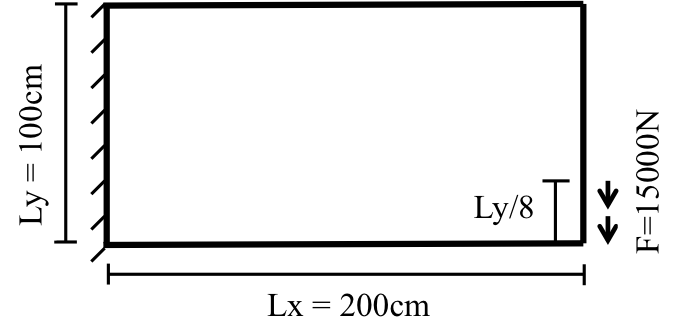
\includegraphics[width=0.6\textwidth]{./figs/newres2/struct.png}
  \caption{Plate thickness design problem}
  \label{fig:struct}
\end{figure}

The response of the plate to the applied force is modeled using the equations of
linear elasticity assuming 2D plane stress.  The governing equations are
discretized using the finite element method with bilinear elements.
A uniform mesh of $n_x \times n_y$ elements is employed, and the thickness
distribution is piecewise constant over each element.  These thickness values
are taken to be the design variables, so there are $n = n_x n_y$ design
variables.

The formal optimization statement is
\begin{equation*}
  \begin{alignedat}{2}
    \underset{x}{\text{min}} \quad &\textsf{mass}(x) = \sum_{i=1}^{n} m_i x_i, & &\\
    \text{subject to} \quad &\textsf{stress}_i(x) \leq \sigma_{\max}, &
    &\forall\; i = 1,2,\ldots,n \\
      & x_l \leq x_i \leq  x_u, \qquad & &\forall\; i = 1,2,\ldots,n,
  \end{alignedat}
\end{equation*}
where $\textsf{mass}(x)$ is the plate mass, and $\textsf{stress}_{i}(x)$ is the
von Mises stress criterion on the $i$th element. \padd{ The thickness of each element
is bounded by the lower and upper values, $x_l = 0.02$ and $x_u = 0.98$. }  

The mass is a linear function
of the design variables and is given by
\begin{equation*}
  \textsf{mass}(x) = \sum_{i=1}^{n} m_i x_i,
\end{equation*}
where $m_i$ is the mass per unit thickness of the $i$th element of the
structure.
\padd{ The objective function 
$\text{mass}(x)$, is a sum of all the elements' mass. Each element's mass
is a weighted summation of the design variables in a surrounding conic area, 
with the weights determined by $1-\frac{r}{r_0}$ } \todo[inline]{please help me
paraphrase here.  It's directly from reading the code. }

The von Mises stress
criterion on the $i$th element can be expressed as
\begin{equation*}
  \textsf{stress}_i(x) = 1 - u(x)^T \mat{B}_i^T \mat{G} \mat{B}_i u(x),
\end{equation*}
where $\mat{B}_i u(x)$ gives the strain as a function of the displacement,
$u(x)$, and $\mat{G}$ is a positive-definite matrix.  The displacement is a
function of the design variables through the discretized governing equation
\begin{equation*}
  R(x,u) = \mat{K}(x) u - b,
\end{equation*}
where $\mat{K}(x)$ is the stiffness matrix and $b$ is the force vector.

We consider a set of three mesh sizes by varying $n_x$ and $n_y$.  Table
\ref{tab:mesh_sizes} lists the mesh dimensions and number of design variables
for the three cases, which we will refer to as the small, medium, and large
cases.

\begin{table}[tbp]
  \begin{center}
    \caption{Mesh dimensions ($n_x$ and $n_y$), number of design variables ($n =
      n_x n_y$), and size of the approximate SVD preconditioner
      ($n_{\mat{\Sigma}}$) for the plate-thickness optimization
      problem \label{tab:mesh_sizes}}
  \begin{tabular}{ l c c c c}
    \textbf{Case} & $\mathbf{n_x}$  & $\mathbf{n_y}$ & $\mathbf{n}$
    & $\mathbf{{n_{\mat{\Sigma}}}}$
    \\ \hline
    \rule{0ex}{3ex}%
    Small  &   16 & 8  & 128  & 20 \\ 
    Medium &   32 & 16 & 512  & 80 \\  
    Large  &   64 & 32 & 2048 & 320  
  \end{tabular}
  \end{center}
\end{table}

Table~\ref{tab:mesh_sizes} also lists the number of approximate singular values
used in Algorithm~\ref{alg:precond}.  As the number of design variables
increases in this structural optimization problem, the number of singular values
in the SVD approximation also has to increase accordingly, \padd{at about $\frac{1}{6}$
of the number of design variables}.
Figure~\ref{fig:svdrank} shows the convergence history of the Krylov iterative
method applied to \eqref{eq:linsys}.  

\padd{To show the effectiveness of the proposed preconditioner, 
Figure~\ref{fig:svdrank} shows the convergence history of the Krylov
method when the Lanczos-based preconditioner uses 
increasing number of SVD ranks. The KKT system is extracted from 
the first Newton step of the final Corrector phase 
at $\mu = 0$ for the small case. }

\begin{figure}[tbp]
  \centering
  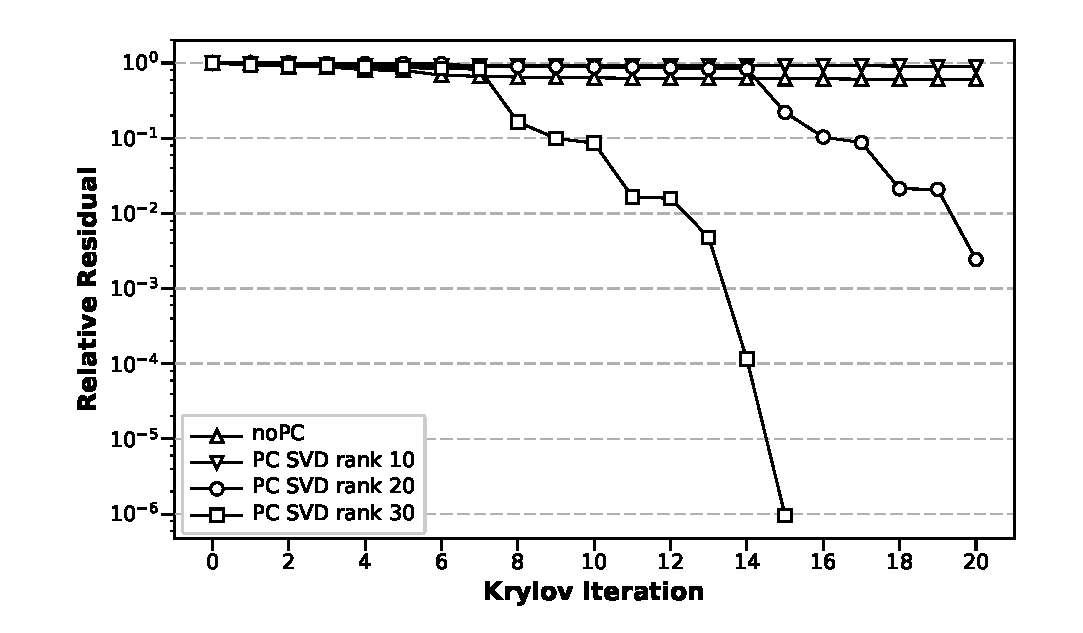
\includegraphics[width=0.7\textwidth]{./figs/newres2/SVD_Ranks.eps}
  \caption{Impact of $\nsig$, the rank of the approximate SVD in
    Algorithm~\ref{alg:precond}, on the Krylov iterative method.
  \label{fig:svdrank}}
\end{figure}

The structural optimization problem was solved using the proposed algorithm,
with and without the preconditioner. Its convergence history were compared with 
that of SNOPT, see Figures \ref{fig:small}, \ref{fig:med}, and \ref{fig:large} for the 
small, medium, and larges cases, respectively. The cost on the horiztonal axis 
measures the equivalent number of PDE solves, 
\ie, the total CPU time divided by the time needed for one
forward solution.  The vertical axis measures the change in relative optimality and
absolute feasiblity.    
  
The final optimal thickness distribution, for the large problem, is plotted in
Figure~\ref{fig:thick}. \padd{The thickness distribution is in agreement with physical
intuition of the problem}. 
  
\begin{figure}[tbp]
  \begin{center}
    \includegraphics*[clip,width=0.8\textwidth]{./figs/newres2/medium_thickness_color.pdf}%
    \caption{Optimal thickness distribution obtained using Algorithm~\ref{alg:pc}.
      \label{fig:thick}}
  \end{center}
\end{figure}  %trim=20 70 0 70, 

The results in Figure~\ref{fig:struct2} highlight the need for preconditioning
on this particular problem: without the approximate-SVD preconditioner the
proposed algorithm is ineffective. 
In contrast, when the approximate-SVD preconditioner is effective, the
proposed inequality optimization algorithm can successfully reduce the optimality 
and feasibility to the desired tolerance.

Figures \ref{fig:small}--\ref{fig:large} also show that the performance of SNOPT
degrades as the problem size increases; on the small problem, optimality is
reduced by only three orders of magnitude, while on the large problem the optimality
fluctuates and struggles to come down.  The feasibility achieved by SNOPT is somewhat better
than its optimality, but it also degrades with problem size.  The proposed
predictor-corrector algorithm is able to converge the optimality and feasiblity
$10^{-5}$ orders of magnitude on all three problems. We see that the
optimization cost increases approximately linearly with problem size on this
problem, and the cost is driven primarily by the increasing number of singular values used
in the preconditioner. 

\begin{figure}[tbp]
  \centering
   \subfloat[small \label{fig:small}]{
   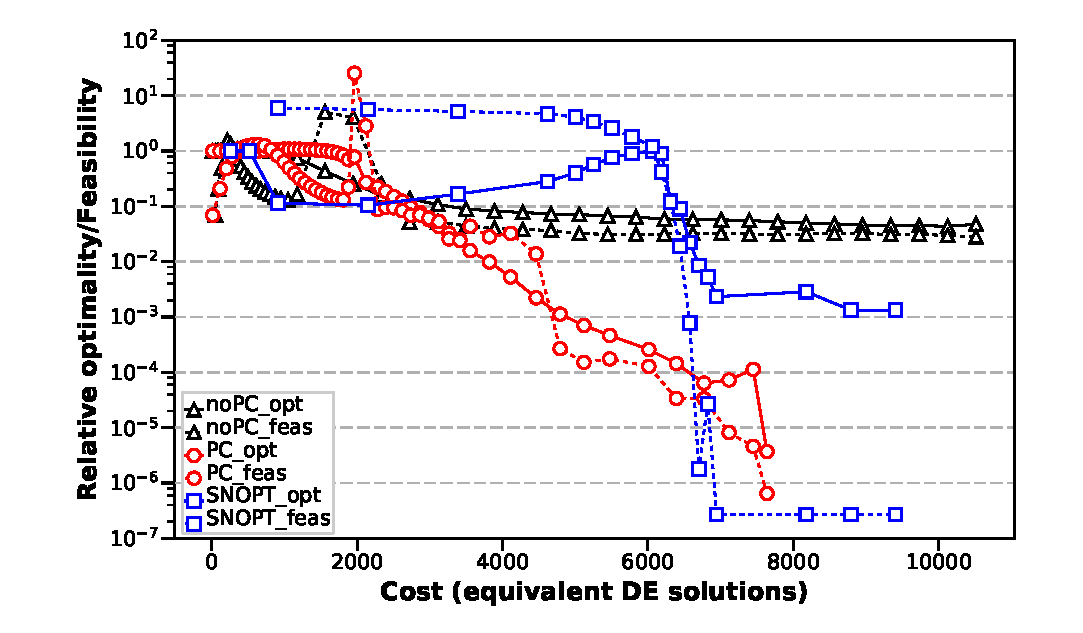
\includegraphics[clip,width=0.75\textwidth]{./figs/newres2/tiny_color.eps} }
  \hspace{1em}
  \subfloat[medium \label{fig:med}]{
   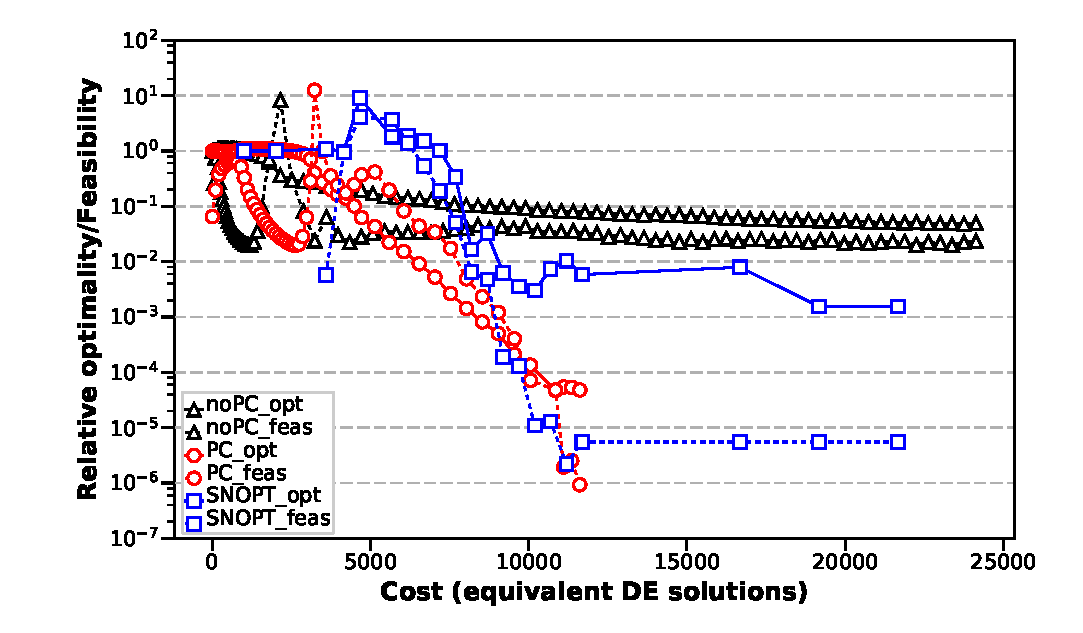
\includegraphics[clip,width=0.75\textwidth]{./figs/newres2/small_color.eps} }
  \hspace{1em}
    \subfloat[large \label{fig:large}]{
   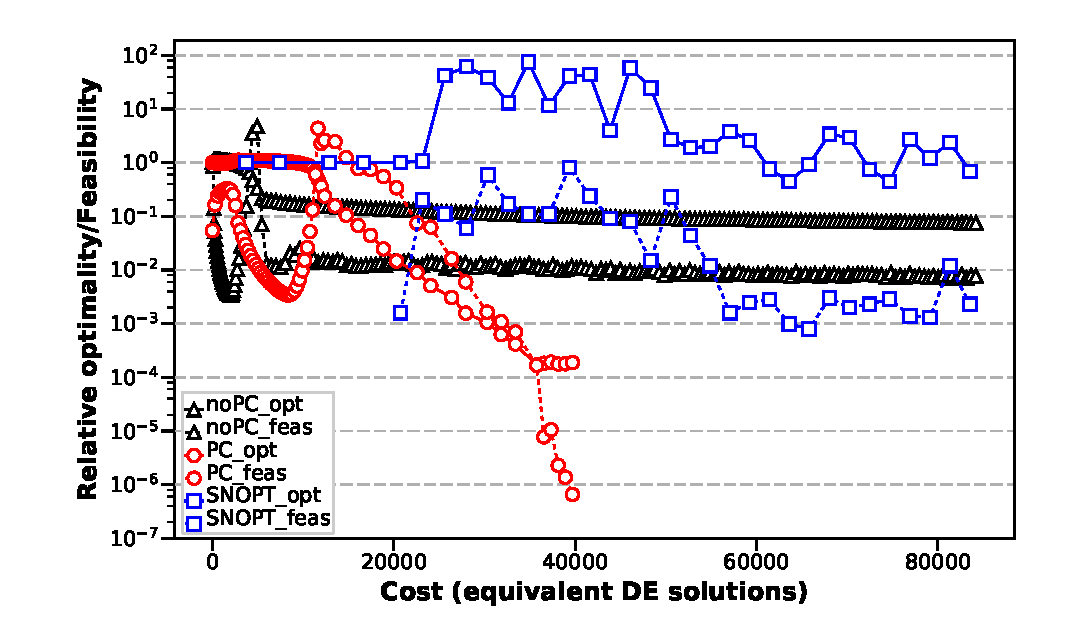
\includegraphics[clip,width=0.75\textwidth]{./figs/newres2/medium_color.eps} }
    \caption{Convergence histories for the three sizes of the structural
      optimization problem. \label{fig:struct2}}
\end{figure}

%%%%%%%%%%%%%%%%%%%%%%%%%%%%%%%%%%%%

%%% Local Variables: 
%%% mode: latex
%%% TeX-master: t
%%% End: 
